\chapter{Recorrido de grafos}

Este capítulo discute dos algoritmos de grafos fundamentales:
búsqueda en profundidad y búsqueda en amplitud.
Ambos algoritmos se dan un nodo de inicio
en el gráfico,
y visitan todos los nodos que se pueden alcanzar
desde el nodo de inicio.
La diferencia en los algoritmos es el orden
en el que visitan los nodos.

\section{Búsqueda en profundidad}

\index{búsqueda en profundidad}

\key{Búsqueda en profundidad} (DFS)
es una técnica de recorrido de grafos sencilla.
El algoritmo comienza en un nodo de inicio,
y procede a todos los demás nodos que son
alcanzables desde el nodo de inicio usando
los bordes del grafo.

La búsqueda en profundidad siempre sigue un solo
camino en el grafo mientras encuentre
nuevos nodos.
Después de esto, regresa a los nodos anteriores
y comienza a explorar otras partes del grafo.
El algoritmo lleva un registro de los nodos visitados,
para que procese cada nodo solo una vez.

\subsubsection*{Ejemplo}

Consideremos cómo la búsqueda en profundidad procesa
el siguiente gráfico:
\begin{center}
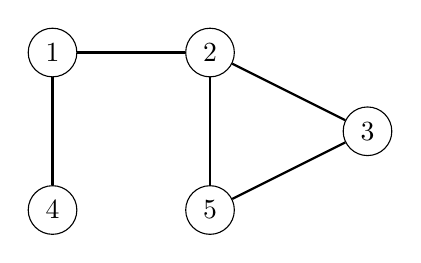
\begin{tikzpicture}
\node[draw, circle] (1) at (1,5) {$1$};
\node[draw, circle] (2) at (3,5) {$2$};
\node[draw, circle] (3) at (5,4) {$3$};
\node[draw, circle] (4) at (1,3) {$4$};
\node[draw, circle] (5) at (3,3) {$5$};

\path[draw,thick,-] (1) -- (2);
\path[draw,thick,-] (2) -- (3);
\path[draw,thick,-] (1) -- (4);
\path[draw,thick,-] (3) -- (5);
\path[draw,thick,-] (2) -- (5);
\end{tikzpicture}
\end{center}
Podemos comenzar la búsqueda en cualquier nodo del gráfico;
ahora comenzaremos la búsqueda en el nodo 1.

La búsqueda primero procede al nodo 2:
\begin{center}
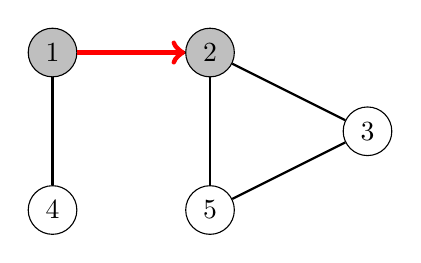
\begin{tikzpicture}
\node[draw, circle,fill=lightgray] (1) at (1,5) {$1$};
\node[draw, circle,fill=lightgray] (2) at (3,5) {$2$};
\node[draw, circle] (3) at (5,4) {$3$};
\node[draw, circle] (4) at (1,3) {$4$};
\node[draw, circle] (5) at (3,3) {$5$};

\path[draw,thick,-] (1) -- (2);
\path[draw,thick,-] (2) -- (3);
\path[draw,thick,-] (1) -- (4);
\path[draw,thick,-] (3) -- (5);
\path[draw,thick,-] (2) -- (5);

\path[draw=red,thick,->,line width=2pt] (1) -- (2);
\end{tikzpicture}
\end{center}
Después de esto, se visitarán los nodos 3 y 5:
\begin{center}
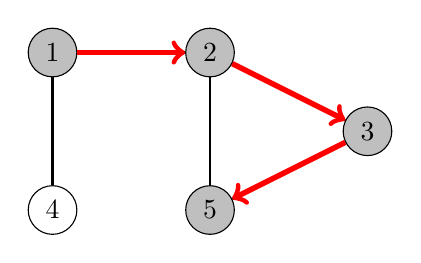
\begin{tikzpicture}
\node[draw, circle,fill=lightgray] (1) at (1,5) {$1$};
\node[draw, circle,fill=lightgray] (2) at (3,5) {$2$};
\node[draw, circle,fill=lightgray] (3) at (5,4) {$3$};
\node[draw, circle] (4) at (1,3) {$4$};
\node[draw, circle,fill=lightgray] (5) at (3,3) {$5$};

\path[draw,thick,-] (1) -- (2);
\path[draw,thick,-] (2) -- (3);
\path[draw,thick,-] (1) -- (4);
\path[draw,thick,-] (3) -- (5);
\path[draw,thick,-] (2) -- (5);

\path[draw=red,thick,->,line width=2pt] (1) -- (2);
\path[draw=red,thick,->,line width=2pt] (2) -- (3);
\path[draw=red,thick,->,line width=2pt] (3) -- (5);
\end{tikzpicture}
\end{center}
Los vecinos del nodo 5 son 2 y 3,
pero la búsqueda ya ha visitado ambos,
por lo que es hora de volver a los nodos anteriores.
También los vecinos de los nodos 3 y 2
han sido visitados, por lo que luego nos movemos
desde el nodo 1 al nodo 4:
\begin{center}
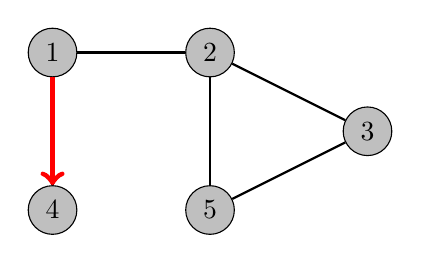
\begin{tikzpicture}
\node[draw, circle,fill=lightgray] (1) at (1,5) {$1$};
\node[draw, circle,fill=lightgray] (2) at (3,5) {$2$};
\node[draw, circle,fill=lightgray] (3) at (5,4) {$3$};
\node[draw, circle,fill=lightgray] (4) at (1,3) {$4$};
\node[draw, circle,fill=lightgray] (5) at (3,3) {$5$};

\path[draw,thick,-] (1) -- (2);
\path[draw,thick,-] (2) -- (3);
\path[draw,thick,-] (1) -- (4);
\path[draw,thick,-] (3) -- (5);
\path[draw,thick,-] (2) -- (5);

\path[draw=red,thick,->,line width=2pt] (1) -- (4);
\end{tikzpicture}
\end{center}
Después de esto, la búsqueda termina porque ha visitado
todos los nodos.

La complejidad temporal de la búsqueda en profundidad es $O(n+m)$
donde $n$ es el número de nodos y $m$ es el
número de bordes,
porque el algoritmo procesa cada nodo y borde una vez.

\subsubsection*{Implementación}

La búsqueda en profundidad se puede implementar convenientemente
utilizando recursión.
La siguiente función \texttt{dfs} comienza
una búsqueda en profundidad en un nodo dado.
La función asume que el gráfico está
almacenado como listas de adyacencia en una matriz
\begin{lstlisting}
vector<int> adj[N];
\end{lstlisting}
y también mantiene una matriz
\begin{lstlisting}
bool visited[N];
\end{lstlisting}
que lleva un registro de los nodos visitados.
Inicialmente, cada valor de la matriz es \texttt{false},
y cuando la búsqueda llega al nodo $s$,
el valor de \texttt{visited}[$s$] se convierte en \texttt{true}.
La función se puede implementar de la siguiente manera:
\begin{lstlisting}
void dfs(int s) {
    if (visited[s]) return;
    visited[s] = true;
    // procesar nodo s
    for (auto u: adj[s]) {
        dfs(u);
    }
}
\end{lstlisting}

\section{Búsqueda en amplitud}

\index{búsqueda en amplitud}

\key{Búsqueda en amplitud} (BFS) visita los nodos
en orden creciente de su distancia
desde el nodo de inicio.
Por lo tanto, podemos calcular la distancia
desde el nodo de inicio a todos los demás
nodos utilizando la búsqueda en amplitud.
Sin embargo, la búsqueda en amplitud es más difícil
de implementar que la búsqueda en profundidad.



La búsqueda en amplitud recorre los nodos
un nivel después de otro.
Primero, la búsqueda explora los nodos cuyo
distancia del nodo de inicio es 1,
luego los nodos cuya distancia es 2, y así sucesivamente.
Este proceso continúa hasta que todos los nodos
han sido visitados.

\subsubsection*{Ejemplo}

Consideremos cómo la búsqueda en amplitud procesa
el siguiente gráfico:

\begin{center}
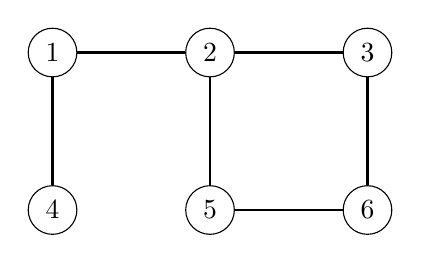
\begin{tikzpicture}
\node[draw, circle] (1) at (1,5) {$1$};
\node[draw, circle] (2) at (3,5) {$2$};
\node[draw, circle] (3) at (5,5) {$3$};
\node[draw, circle] (4) at (1,3) {$4$};
\node[draw, circle] (5) at (3,3) {$5$};
\node[draw, circle] (6) at (5,3) {$6$};

\path[draw,thick,-] (1) -- (2);
\path[draw,thick,-] (2) -- (3);
\path[draw,thick,-] (1) -- (4);
\path[draw,thick,-] (3) -- (6);
\path[draw,thick,-] (2) -- (5);
\path[draw,thick,-] (5) -- (6);
\end{tikzpicture}
\end{center}
Supongamos que la búsqueda comienza en el nodo 1.
Primero, procesamos todos los nodos que se pueden alcanzar
desde el nodo 1 usando un solo borde:
\begin{center}
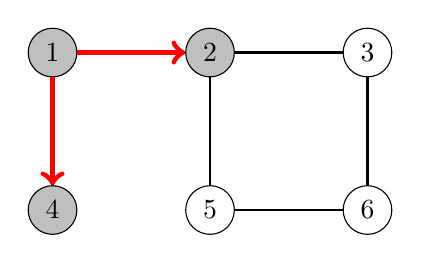
\begin{tikzpicture}
\node[draw, circle,fill=lightgray] (1) at (1,5) {$1$};
\node[draw, circle,fill=lightgray] (2) at (3,5) {$2$};
\node[draw, circle] (3) at (5,5) {$3$};
\node[draw, circle,fill=lightgray] (4) at (1,3) {$4$};
\node[draw, circle] (5) at (3,3) {$5$};
\node[draw, circle] (6) at (5,3) {$6$};

\path[draw,thick,-] (1) -- (2);
\path[draw,thick,-] (2) -- (3);
\path[draw,thick,-] (1) -- (4);
\path[draw,thick,-] (3) -- (6);
\path[draw,thick,-] (2) -- (5);
\path[draw,thick,-] (5) -- (6);

\path[draw,thick,-] (1) -- (2);
\path[draw,thick,-] (2) -- (3);
\path[draw,thick,-] (1) -- (4);
\path[draw,thick,-] (2) -- (5);

\path[draw=red,thick,->,line width=2pt] (1) -- (2);
\path[draw=red,thick,->,line width=2pt] (1) -- (4);
\end{tikzpicture}
\end{center}
Después de esto, procedemos a los nodos 3 y 5:
\begin{center}
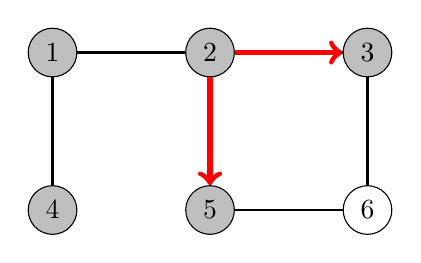
\begin{tikzpicture}
\node[draw, circle,fill=lightgray] (1) at (1,5) {$1$};
\node[draw, circle,fill=lightgray] (2) at (3,5) {$2$};
\node[draw, circle,fill=lightgray] (3) at (5,5) {$3$};
\node[draw, circle,fill=lightgray] (4) at (1,3) {$4$};
\node[draw, circle,fill=lightgray] (5) at (3,3) {$5$};
\node[draw, circle] (6) at (5,3) {$6$};

\path[draw,thick,-] (1) -- (2);
\path[draw,thick,-] (2) -- (3);
\path[draw,thick,-] (1) -- (4);
\path[draw,thick,-] (3) -- (6);
\path[draw,thick,-] (2) -- (5);
\path[draw,thick,-] (5) -- (6);

\path[draw,thick,-] (1) -- (2);
\path[draw,thick,-] (2) -- (3);
\path[draw,thick,-] (1) -- (4);
\path[draw,thick,-] (2) -- (5);

\path[draw=red,thick,->,line width=2pt] (2) -- (3);
\path[draw=red,thick,->,line width=2pt] (2) -- (5);
\end{tikzpicture}
\end{center}
Finalmente, visitamos el nodo 6:
\begin{center}
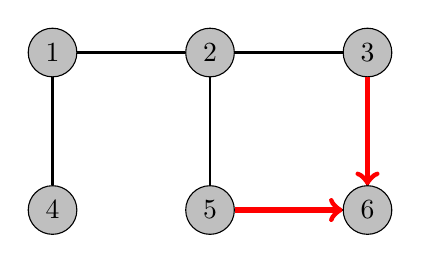
\begin{tikzpicture}
\node[draw, circle,fill=lightgray] (1) at (1,5) {$1$};
\node[draw, circle,fill=lightgray] (2) at (3,5) {$2$};
\node[draw, circle,fill=lightgray] (3) at (5,5) {$3$};
\node[draw, circle,fill=lightgray] (4) at (1,3) {$4$};
\node[draw, circle,fill=lightgray] (5) at (3,3) {$5$};
\node[draw, circle,fill=lightgray] (6) at (5,3) {$6$};

\path[draw,thick,-] (1) -- (2);
\path[draw,thick,-] (2) -- (3);
\path[draw,thick,-] (1) -- (4);
\path[draw,thick,-] (3) -- (6);
\path[draw,thick,-] (2) -- (5);
\path[draw,thick,-] (5) -- (6);

\path[draw,thick,-] (1) -- (2);
\path[draw,thick,-] (2) -- (3);
\path[draw,thick,-] (1) -- (4);
\path[draw,thick,-] (2) -- (5);

\path[draw=red,thick,->,line width=2pt] (3) -- (6);
\path[draw=red,thick,->,line width=2pt] (5) -- (6);
\end{tikzpicture}
\end{center}
Ahora hemos calculado las distancias
desde el nodo de inicio a todos los nodos del gráfico.
Las distancias son las siguientes:

\begin{tabular}{ll}
\\
nodo & distancia \\
\hline
1 & 0 \\
2 & 1 \\
3 & 2 \\
4 & 1 \\
5 & 2 \\
6 & 3 \\
\\
\end{tabular}

Al igual que en la búsqueda en profundidad,
la complejidad temporal de la búsqueda en amplitud
es $O(n+m)$, donde $n$ es el número de nodos
y $m$ es el número de aristas.

\subsubsection*{Implementación}

La búsqueda en amplitud es más difícil
de implementar que la búsqueda en profundidad,
porque el algoritmo visita nodos
en diferentes partes del gráfico.
Una implementación típica se basa en
una cola que contiene nodos.
En cada paso, el siguiente nodo en la cola
será procesado.

El siguiente código asume que el gráfico se almacena
como listas de adyacencia y mantiene las siguientes
estructuras de datos:
\begin{lstlisting}
queue<int> q;
bool visited[N];
int distance[N];
\end{lstlisting}

La cola \texttt{q}
contiene nodos a procesar
en orden creciente de su distancia.
Los nuevos nodos siempre se agregan al final
de la cola, y el nodo al principio
de la cola es el siguiente nodo a procesar.
La matriz \texttt{visited} indica
qué nodos la búsqueda ya ha visitado,
y la matriz \texttt{distance} contendrá la
distancias desde el nodo de inicio a todos los nodos del gráfico.
La búsqueda se puede implementar de la siguiente manera,
comenzando en el nodo $x$:
\begin{lstlisting}
visited[x] = true;
distance[x] = 0;
q.push(x);
while (!q.empty()) {
    int s = q.front(); q.pop();
    // process node s
    for (auto u : adj[s]) {
        if (visited[u]) continue;
        visited[u] = true;
        distance[u] = distance[s]+1;
        q.push(u);
    }
}
\end{lstlisting}

\section{Aplicaciones}

Usando los algoritmos de recorrido de grafos,
podemos verificar muchas propiedades de los grafos.
Por lo general, tanto la búsqueda en profundidad como
la búsqueda en anchura se pueden utilizar,
pero en la práctica, la búsqueda en profundidad
es una mejor opción, porque es
más fácil de implementar.
En las siguientes aplicaciones asumiremos que
el grafo no está dirigido.

\subsubsection{Verificación de conectividad}

\index{grafo conectado}

Un grafo está conectado si hay un camino
entre dos nodos cualesquiera del grafo.
Por lo tanto, podemos verificar si un grafo está conectado
comenzando en un nodo arbitrario y
averiguando si podemos llegar a todos los demás nodos.

Por ejemplo, en el grafo
\begin{center}
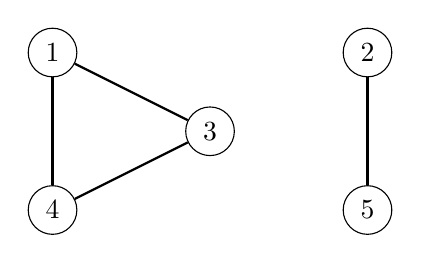
\begin{tikzpicture}
\node[draw, circle] (2) at (7,5) {$2$};
\node[draw, circle] (1) at (3,5) {$1$};
\node[draw, circle] (3) at (5,4) {$3$};
\node[draw, circle] (5) at (7,3) {$5$};
\node[draw, circle] (4) at (3,3) {$4$};

\path[draw,thick,-] (1) -- (3);
\path[draw,thick,-] (1) -- (4);
\path[draw,thick,-] (3) -- (4);
\path[draw,thick,-] (2) -- (5);
\end{tikzpicture}
\end{center}
una búsqueda en profundidad desde el nodo $1$ visita
los siguientes nodos:
\begin{center}
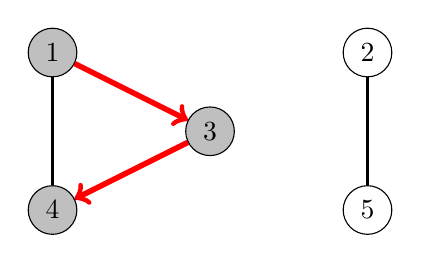
\begin{tikzpicture}
\node[draw, circle] (2) at (7,5) {$2$};
\node[draw, circle,fill=lightgray] (1) at (3,5) {$1$};
\node[draw, circle,fill=lightgray] (3) at (5,4) {$3$};
\node[draw, circle] (5) at (7,3) {$5$};
\node[draw, circle,fill=lightgray] (4) at (3,3) {$4$};

\path[draw,thick,-] (1) -- (3);
\path[draw,thick,-] (1) -- (4);
\path[draw,thick,-] (3) -- (4);
\path[draw,thick,-] (2) -- (5);

\path[draw=red,thick,->,line width=2pt] (1) -- (3);
\path[draw=red,thick,->,line width=2pt] (3) -- (4);

\end{tikzpicture}
\end{center}

Como la búsqueda no visitó todos los nodos,
podemos concluir que el grafo no está conectado.
De manera similar, también podemos encontrar todos los componentes conectados
de un grafo iterando a través de los nodos y siempre
comenzando una nueva búsqueda en profundidad si el nodo actual
no pertenece a ningún componente todavía.

\subsubsection{Encontrar ciclos}

\index{ciclo}

Un grafo contiene un ciclo si durante un recorrido del grafo,
encontramos un nodo cuyo vecino (diferente del
nodo anterior en la ruta actual) ya ha sido
visitado.
Por ejemplo, el grafo
\begin{center}
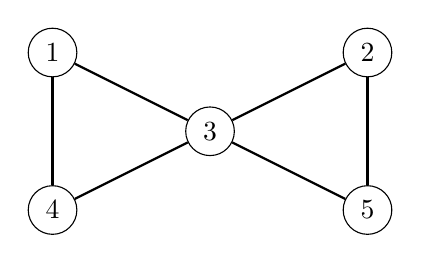
\begin{tikzpicture}
\node[draw, circle] (2) at (7,5) {$2$};
\node[draw, circle] (1) at (3,5) {$1$};
\node[draw, circle] (3) at (5,4) {$3$};
\node[draw, circle] (5) at (7,3) {$5$};
\node[draw, circle] (4) at (3,3) {$4$};

\path[draw,thick,-] (1) -- (3);
\path[draw,thick,-] (1) -- (4);
\path[draw,thick,-] (3) -- (4);
\path[draw,thick,-] (2) -- (5);
\path[draw,thick,-] (2) -- (3);
\path[draw,thick,-] (3) -- (5);
\end{tikzpicture}
\end{center}
contiene dos ciclos y podemos encontrar uno
de ellos de la siguiente manera:
\begin{center}
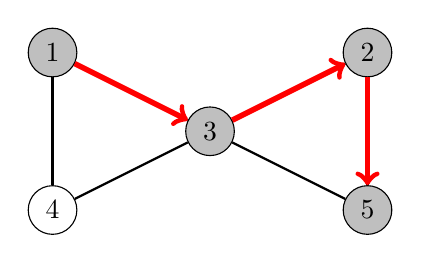
\begin{tikzpicture}
\node[draw, circle,fill=lightgray] (2) at (7,5) {$2$};
\node[draw, circle,fill=lightgray] (1) at (3,5) {$1$};
\node[draw, circle,fill=lightgray] (3) at (5,4) {$3$};
\node[draw, circle,fill=lightgray] (5) at (7,3) {$5$};
\node[draw, circle] (4) at (3,3) {$4$};

\path[draw,thick,-] (1) -- (3);
\path[draw,thick,-] (1) -- (4);
\path[draw,thick,-] (3) -- (4);
\path[draw,thick,-] (2) -- (5);
\path[draw,thick,-] (2) -- (3);
\path[draw,thick,-] (3) -- (5);

\path[draw=red,thick,->,line width=2pt] (1) -- (3);
\path[draw=red,thick,->,line width=2pt] (3) -- (2);
\path[draw=red,thick,->,line width=2pt] (2) -- (5);

\end{tikzpicture}
\end{center}
Después de movernos del nodo 2 al nodo 5, notamos que
el vecino 3 del nodo 5 ya ha sido visitado.
Por lo tanto, el grafo contiene un ciclo que pasa por el nodo 3,
por ejemplo, $3 \rightarrow 2 \rightarrow 5 \rightarrow 3$.

Otra forma de averiguar si un grafo contiene un ciclo
es simplemente calcular el número de nodos y aristas
en cada componente.
Si un componente contiene $c$ nodos y no ciclo,
debe contener exactamente $c-1$ aristas
(por lo que tiene que ser un árbol).
Si hay $c$ o más aristas, el componente
seguramente contiene un ciclo.

\subsubsection{Verificación de bipartición}

\index{grafo bipartito}

Un grafo es bipartito si sus nodos se pueden colorear
usando dos colores de modo que no haya nodos adyacentes
con el mismo color.
Es sorprendentemente fácil comprobar si un grafo
es bipartito utilizando algoritmos de recorrido del grafo.

La idea es colorear el nodo inicial de azul,
todos sus vecinos de rojo, todos sus vecinos de azul, y así sucesivamente.
Si en algún momento de la búsqueda notamos que
dos nodos adyacentes tienen el mismo color,
esto significa que el grafo no es bipartito.
De lo contrario, el grafo es bipartito y se ha encontrado una coloración.


Por ejemplo, el gráfico
\begin{center}
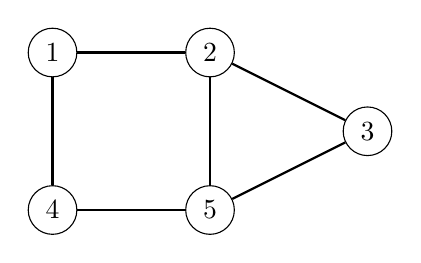
\begin{tikzpicture}
\node[draw, circle] (2) at (5,5) {$2$};
\node[draw, circle] (1) at (3,5) {$1$};
\node[draw, circle] (3) at (7,4) {$3$};
\node[draw, circle] (5) at (5,3) {$5$};
\node[draw, circle] (4) at (3,3) {$4$};

\path[draw,thick,-] (1) -- (2);
\path[draw,thick,-] (2) -- (5);
\path[draw,thick,-] (5) -- (4);
\path[draw,thick,-] (4) -- (1);
\path[draw,thick,-] (2) -- (3);
\path[draw,thick,-] (5) -- (3);
\end{tikzpicture}
\end{center}
no es bipartito, porque una búsqueda desde el nodo 1
procede de la siguiente manera:
\begin{center}
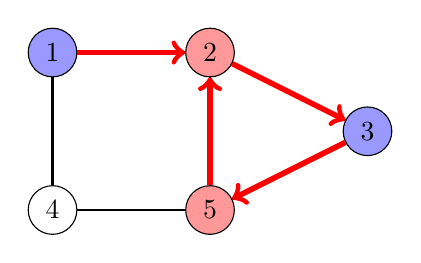
\begin{tikzpicture}
\node[draw, circle,fill=red!40] (2) at (5,5) {$2$};
\node[draw, circle,fill=blue!40] (1) at (3,5) {$1$};
\node[draw, circle,fill=blue!40] (3) at (7,4) {$3$};
\node[draw, circle,fill=red!40] (5) at (5,3) {$5$};
\node[draw, circle] (4) at (3,3) {$4$};

\path[draw,thick,-] (1) -- (2);
\path[draw,thick,-] (2) -- (5);
\path[draw,thick,-] (5) -- (4);
\path[draw,thick,-] (4) -- (1);
\path[draw,thick,-] (2) -- (3);
\path[draw,thick,-] (5) -- (3);

\path[draw=red,thick,->,line width=2pt] (1) -- (2);
\path[draw=red,thick,->,line width=2pt] (2) -- (3);
\path[draw=red,thick,->,line width=2pt] (3) -- (5);
\path[draw=red,thick,->,line width=2pt] (5) -- (2);
\end{tikzpicture}
\end{center}
Observamos que el color de ambos nodos 2 y 5
es rojo, mientras que son nodos adyacentes en el gráfico.
Por lo tanto, el gráfico no es bipartito.

Este algoritmo siempre funciona, porque cuando hay
solo dos colores disponibles,
el color del nodo de inicio en un componente
determina los colores de todos los demás nodos en el componente.
No importa si el
nodo de inicio es rojo o azul.

Tenga en cuenta que en el caso general,
es difícil averiguar si los nodos
en un gráfico se pueden colorear usando $k$ colores
de modo que ningún nodo adyacente tenga el mismo color.
Incluso cuando $k=3$, no se conoce ningún algoritmo eficiente
pero el problema es NP-difícil.
